\subsubsection{Gamification} \label{background_gamemechanics}
Gamification is a relatively new area of interest, and has become particularly
popular with online businesses seeking to increase customer engagement\cite{_farmville_2010}. Several
new companies have formed (BigDoor, BunchBall, BadgeVille) which provide turnkey
solutions to `gamify' a web site in the hopes that customer engagement will 
increase and thereby drive revenue. BigDoor for example claims a 3 times 
engagement lift and a 7 times increase
in revenue per user when applying their gamification system\cite{_bigdoor_????}.

Gamification does not necessarily mean converting an application to look and feel like a game with elements such as sound effects and graphics, but instead usually involves
taking elements of games (game mechanics) such as a scoring system and applying them to
non game environments \cite{carr_gamification:_2011}.

Thomas Malone suggested that there several elements \cite{malone_what_1980} in computer games which make them engaging -- namely the following.
\paragraph{Goals}
Games should have goals with feedback as to how close the user is to reaching
the goal.
Some of the elements that people mention\cite{csikszentmihalyi_flow:_1991} when they are enjoying a task with a particular goal are:
\begin{itemize}
	\item The goal of the task is clear.
	\item Immediate feedback is given by the task.
	\item The goal is achievable.
	\item The person has control over the task.
\end{itemize}

\paragraph{Uncertain Outcomes}
By making outcomes uncertain, a dynamic is added which gives the player a sense
of discovery and removes monotony.
\paragraph{Self-esteem}
Success results in a boost of self-esteem for students, while failure can
result in a loss of self-esteem. Therefore it is important to have a balance
such that the user can complete challenges which are difficult enough that they
will feel accomplishment without making the challenges too difficult that they
lose confidence.
\paragraph{Intrinsic and Extrinsic Fantasies}
Extrinsic fantasies involve a story which is unrelated to the learning material
or skills being learned, however the skills are required to progress through the
story. In contrast, an intrinsic fantasy involves the skills within the story,
where the skills are required not only to progress through the story, but to
understand the story. In this sense intrinsic fantasies are intertwined in the
skills themselves and provide a more believable real-world usage, rather than 
being simply layered on top with no relation to the skills.
\paragraph{Sensory Curiosity}
Generally in the form of sound and graphics associated with rewards, fantasy or
just to enhance the overall experience.
\paragraph{Cognitive Curiosity}
The desire to complete and draw connections between the learner's knowledge and
cognitive structures.
\paragraph{Informative Feedback} Making environments responsive to the user's actions.
Feedback might be both surprising and constructive. By giving feedback in unexpected
places, the user will be left to discover the environment on their own. Constructive
feedback should inform users where their knowledge is incomplete and how to change
their knowledge.
\subsubsection{Extrinsic vs. Intrinsic Motivation}
Motivation is often classified as one of two categories by dualists - Extrinsic and Intrinsic motivation. Intrinsic motivation refers to the motivation one feels for a task when that person feels that completing the task is enjoyable or fulfilling. Extrinsic motivation refers to motivation due to an external factor, usually a reward such as money.

It is difficult to classify
rewards in games into either instrinsic or extrinsic motivation. In a sense the 
`reward' game mechanic would at first appear to be an extrinsic motivation.
However, rewards in games are interesting because for most games, the reward is not tangible.
In fact in many cases the opposite is true.
The FarmVille game by Zynga for example accepts money from its users who wish to purchase
in-game credits, however those in-game credits cannot be exchanged for anything
tangible \cite{gabe_zichermann_fun_2010}. Therefore it could be concluded that
users are playing for their own satisfaction, not to \textit{gain} anything which
seems to be more an element of intrinsic motivation.

\subsubsection{Previous Work}
\paragraph{Khan Academy}
The Khan Academy\cite{_khan_????} is one of the most well known examples of
game elements applied to learning. The Khan Academy hosts over 2,400 videos on various
subjects, provides quizzes and adds game mechanics and rules to the whole learning environment.

In an article about the Khan Academy, Roy Saunderson suggests that the principles
from the Khan Academy could be applied to workplace training \cite{saunderson_making_2011}.
These principles include Goal Focused, Obtaining Feedback, Collecting Points, Reaching
Levels, Own Pace, and Learning Metrics. These principles all match 
in some way with the elements suggested by Malone\cite{malone_what_1980} with
the exception of Learning Metrics.

Learning Metrics is a side benefit of applying a
quantitative scoring system to a learning environment. The system inherently
tracks the progress of students and therefore can provide real-time information
to teaching staff about which students might need support.

\begin{figure}[h]
	\centering
		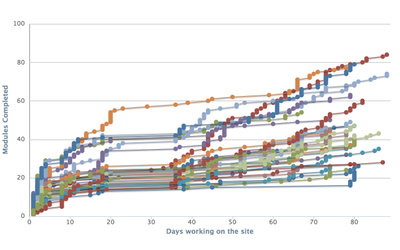
\includegraphics[width=10cm]{./khan.png}    
		\caption{Learning Metrics on Khan Academy shows graphs of student progress}
\end{figure}

\paragraph{socialPsych}
The socialPsych\cite{landers_casual_2011} project examined some game mechanics
with an online social learning environment which was run in parallel to university
courses. The authors of the project compiled a list of best practices
for casual social games used for learning, of which a few are relevant to
the project discussed in this proposal. Immediacy of feedback (in terms of
rewards or validation for completing a task) was found to be important for
motivation \cite[p. 419]{landers_casual_2011}. Game rewards should also be adjusted
to a difficulty which is achievable without being overly easy to ensure the user
feels satisfaction upon completion \cite[p. 420]{landers_casual_2011}.

An interesting result of the socialPsych project was that 29\% of the students
completed multiple choice tests which were completely \textit{optional}\cite[p. 416]{landers_casual_2011}. Student
opinions of the platform regarded it as `fun'\cite[p. 417]{landers_casual_2011}. Some students complained of the
lack of feedback on which answers were correct or incorrect which ties in to
the principle of Informative Feedback proposed by Malone\cite{malone_what_1980}. 

